% ============================================================================
% VALUE-DIRECTED ATTENTION — Validity4 + Baruni (affine_ew model only).
% Companion result to the core-detection section (sec:detection): the
% value-VDA validity is strongest at the cue and weakly recoverable thereafter;
% here we isolate spatial validity and show the model USES it.
% All numbers are the affine_ew ("the model") figures from ACT_II_RESULTS.md
% (II.2 Validity4, II.3 Baruni) and ACT_I_VDA_RESULTS.md §5 (the contrast).
% ============================================================================
\section{Value-directed attention: the model uses spatial validity, but
         in an absolute-value regime}
\label{sec:value}

The core-detection results (Section~\ref{sec:detection}) leave a pointed puzzle.
On the value-directed-attention (VDA) environment the model \emph{perceives} the
predictiveness of the cue --- cue validity is decodable from the working-memory
state at cue onset --- and yet its behavior is validity-flat: the cueing benefit
does not grow as the cue becomes more reliable, and validity is only weakly
recoverable after the first frame (Section~\ref{sec:detection}). Taken alone
this looks like a limitation. This section tests whether the pattern depends on
task regime, using two separately trained manipulations. First, an environment in which spatial validity is the \emph{only}
operative cue --- no competing value colour --- to ask whether the capacity to use
validity is present at all. Second, a relative-value manipulation to ask whether
the model's value sensitivity is context-dependent or absolute. The first is a
positive association: without a competing value cue, the Validity4 checkpoint uses validity gradedly,
in a Posner-like manner \cite{posner1980_orienting}. The second is a principled
null: the model is in an absolute-value regime, consistent with the separate normative account
of when value-directed attention should matter. Together they motivate, but do not
prove, a cue-competition hypothesis for why the value-VDA was validity-flat, and
locate the model precisely within the human and primate literature on spatial
cueing and reward-directed selection.

Throughout, ``the model'' denotes the affine-feedback architecture. Validity4 and
Baruni results are read from separately trained checkpoints, not from the canonical
VDA4 weights reported in Section~\ref{sec:detection}; they share the analysis harness.

% ----------------------------------------------------------------------------
\subsection{Validity4: spatial validity, used gradedly}
\label{sec:value-validity4}
% FIGURE: validity4_curves.png (from validity4_repro.py):
%   (a) cueing benefit (cued - uncued detection) vs validity 25/50/75/100%,
%   (b) uncued detection vs validity, (c) cued-patch attention alpha1 vs
%   validity, all at Delta=26. affine_ew curves only.
\begin{figure}[t]\centering
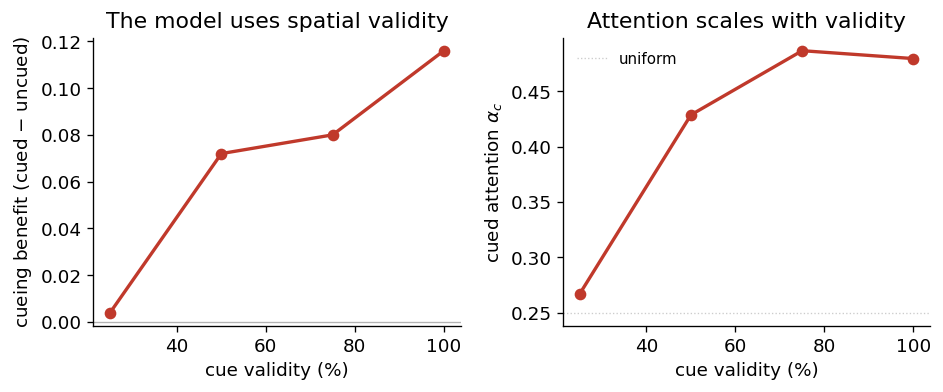
\includegraphics[width=0.92\textwidth]{figures/fig_value_validity4.png}
\caption{\textbf{A separately trained Validity4 checkpoint uses spatial validity.} With no competing value cue, the
cueing benefit (cued $-$ uncued detection at $\Delta=26^\circ$; left) grows
monotonically with cue validity, and cued-patch attention $\alpha_c$ (right) rises
from near the uniform baseline ($0.25$) toward $0.48$ as the ring signals higher
reliability. Curves are the model (affine feedback).}
\label{fig:validity4}
\end{figure}

The cue is a white ring around
the candidate location, and the \emph{completeness} of that ring is the displayed
validity level. This legacy Validity4 checkpoint uses a four-location target sampler
that can return to the cue on the nominally invalid branch, so its realized
cued-change probability is $p+(1-p)/4$: displayed $p=0.25$ realizes $0.4375$.
It is therefore the lowest displayed-validity condition, not an uninformative or
chance cue. Crucially there is no value colour: nothing on the cue signals worth,
so displayed validity is the single cue dimension the model could exploit.
This is a separately trained complement to the value-VDA of
Section~\ref{sec:detection}, where a value cue and a validity cue share the display.

Freed of the competing value signal, the model uses validity, and it uses it
\emph{gradedly}. Three converging measures, all read at a fixed change magnitude
$\Delta = 26$, establish the effect.

\paragraph{The cueing benefit grows monotonically with validity.} The spatial-cueing
benefit --- detection at the cued location minus detection at an uncued location ---
rises monotonically across displayed ring levels: it is essentially absent
at the lowest displayed level and opens to a clear benefit when the cue is fully
valid ($0.00 \to 0.07 \to 0.08 \to 0.12$ across validity $25\% \to 50\% \to 75\%
\to 100\%$). This is a Posner-like graded cueing effect under the legacy sampler
\cite{posner1980_orienting}: performance at the cued location improves across
displayed ring levels.
It also provides a cross-checkpoint contrast with the value-VDA checkpoint, where
validity is present alongside value but has little measurable control over deployment
(Section~\ref{sec:detection}). Because the checkpoints were trained separately, the
contrast shows that the architecture can learn to act on cue predictiveness when it is
the only operative cue. It does not isolate cue removal within fixed weights. Validity4
and archived VDA4 use the same legacy four-location target rule, so target semantics do
not confound this pair; separate training and the presence versus absence of the value
cue still confound the cross-checkpoint interpretation.

\paragraph{Uncued detection falls as validity rises --- a pattern compatible with a resource trade-off.}
The benefit is not merely a gain added at the cued location on top of an unchanged
baseline. As the cue becomes more predictive the model \emph{withdraws} from the
uncued locations: detection at uncued locations falls from $0.94$ at the
lowest displayed-validity cue to $0.86$ at the fully valid cue. The paired decrease is compatible with monitoring being diverted
away from where the cue says a change is less likely and toward where it says a change
is likely. It supports, but does not uniquely identify, reallocation of a limited
attentional resource rather than a one-sided cued enhancement
\cite{posner1980_orienting, MullerFindlay1987}. A pure criterion shift at the cued
location would leave uncued performance untouched; the falling uncued detection
shows a genuine redistribution of processing, consistent with a normalization-style
competition in which enhancing one location suppresses the others
\cite{reynolds_heeger2009_normalization}.

\paragraph{Cued-patch attention rises with validity.} The behavioral trade-off has
a direct correlate in the model's internal attention. The fraction of attention the
model places on the cued patch, $\alpha_1$ (uniform allocation over the four
locations $= 0.25$), rises with displayed validity from $0.27$ --- barely above uniform at
the lowest displayed level --- to $0.48$ when the cue is fully valid. The checkpoint assigns more priority to the cued patch when the ring indicates higher
reliability. This covaries with the behavioral cueing effect: a
graded, validity-scaled deployment of the priority map, the model analogue of the
graded top-down enhancement that spatial cues elicit in visual cortex
\cite{mcadams_maunsell1999_v4_tuning, reynolds_heeger2009_normalization,
carrasco2011_visual_attention_25y}. That the same manipulation moves behavior
(cueing benefit), the neglected alternative (uncued detection), and the internal
allocation ($\alpha_1$) in register supports a reallocation interpretation within
this checkpoint, while the cross-checkpoint comparison remains correlational.

Taken together the three measures are a graded, Posner-like validity effect
\cite{posner1980_orienting}: the more predictive the cue, the larger the cued
benefit, the larger the uncued cost, and the more attention the model commits to the
cued location. The model does not merely orient to \emph{where} it is told to look;
when validity is the operative cue it is sensitive to \emph{how much} the cue can be
trusted --- the parametric dependence that was absent in the value-VDA.

% ----------------------------------------------------------------------------
\subsection{The contrast with the value-VDA: a cue-competition hypothesis}
\label{sec:value-crowdout}
% FIGURE: reuse decode_curves (sec:detection) — canonical VDA4 validity is
% 0.773 at t1, 0.296 at t2, and weak thereafter (mean t2--t6 0.309) — placed
% beside validity4_curves to contrast weak post-cue recoverability with use.

The Validity4 result acquires its force from the contrast with the value-VDA of
Section~\ref{sec:detection}. There, on a cue ring that \emph{also} carried a value
colour, the model's measured cueing benefit was nearly flat across displayed
validity. In the value-VDA, displayed validity was most decodable from the working-memory
state at cue onset ($0.773$ at $t=1$), then fell near chance at the blank
($0.296$ at $t=2$) and remained weak thereafter (mean $t=2$--$6$: $0.309$)
(Section~\ref{sec:detection}). The probe therefore shows strongest recoverability at
the cue and only weak post-cue recoverability; it does not by itself establish active
discarding.

Validity4 supplies a complementary, target-rule-matched but separately trained result. The architecture
can use displayed validity when it is the only cue and can act on it gradedly
(Section~\ref{sec:value-validity4}); both it and archived VDA4 use the legacy
four-location sampler. One interpretation is that a value cue competes
with validity for maintained control in the value-VDA. This cue-competition account is
consistent with the reward-directed
selection literature, in which reward-associated features dominate attentional
priority even when other predictive information is available and even when it is
suboptimal to let them do so \cite{failing_theeuwes2018_selection_history,
hickey2010_reward_salience_acc, wang_theeuwes2018_statistical_learning_distractor_suppression}.
The two separately trained environments therefore show that validity use is within the
architecture's repertoire but is not expressed strongly in the canonical value-VDA.
They do not establish monopolization of a fixed memory resource or prove that value
causes validity to be discarded; doing so would require a within-checkpoint cue
intervention or matched retraining controls.

% ----------------------------------------------------------------------------
\subsection{Baruni relative-value: a principled null in the absolute-value regime}
\label{sec:value-baruni}
% FIGURE: baruni_* (from baruni_core.py / baruni_repro.py):
%   high-value vs low-value detection across the relative-value manipulation,
%   plus value-directed-attention (alpha) readout — affine_ew only. Show the
%   flat/weak value curve and the absence of value-directed attention.

The final manipulation asks a different question about value: is the model's value
sensitivity \emph{relative} --- scaled by the local context of available rewards,
as in the primate relative-value paradigm --- or \emph{absolute}? The Baruni test
sets a high-value and a low-value option in the same display and varies their
relative worth. A relative-value system would track the \emph{contrast} between the
options; an absolute-value system would track each option's worth on its own scale.

The model is in the \emph{absolute}-value regime. Its response to the relative-value
manipulation is flat: high-versus-low value does not modulate detection, and there
is no value-directed attention --- no reallocation of the priority map toward the
higher-valued option as its relative worth grows. This is a \emph{null}, and it is
important to read it correctly. It is not a positive relative-value effect. It is
consistent with the separate normative account's high-sensitivity regime, in which
value should be tracked absolutely, not relatively, and value-directed
\emph{attention} should be weak or absent because reallocating
attention by relative value buys little when sensitivity is already high. The Baruni
null is therefore a cross-paper \emph{consistency check}: the absolute-value,
weak-value-directed-attention regime identified by the normative treatment is
compatible with the trained checkpoint
\cite{failing_theeuwes2018_selection_history,morgan_albanna_herman2026_vda}. This
agreement does not make the null a confirmation of the normative theory.

% ----------------------------------------------------------------------------
\subsection{Summary}
\label{sec:value-summary}

The value-directed-attention results resolve the puzzle left by the core detection
battery and place the model in the literature. When spatial validity is the
operative cue, the model uses it gradedly --- a monotone, Posner-like cueing benefit
($0.00 \to 0.12$ across validity), a matching withdrawal from uncued locations
($0.94 \to 0.86$), and a validity-scaled deployment of internal attention
($\alpha_1: 0.27 \to 0.48$) --- reproducing the canonical spatial-cueing effect
\cite{posner1980_orienting, MullerFindlay1987}. That this graded validity use is
weak in the value-VDA motivates a cue-competition hypothesis: a competing value cue
may take precedence while validity drops from maintained memory
(Section~\ref{sec:detection}), consistent with reward-directed selection influencing
attentional priority \cite{failing_theeuwes2018_selection_history,
hickey2010_reward_salience_acc}. And the model tracks value \emph{absolutely}: the
Baruni relative-value manipulation yields a principled null --- flat detection, no
value-directed attention --- consistent with the high-sensitivity regime of the
separate normative account. Across separately trained checkpoints, the architecture
can use spatial validity when validity is the operative cue and can display an
absolute-value regime; causal value-driven crowd-out remains to be tested.
